% CVPR 2027 submission. Style files from https://github.com/cvpr-org/author-kit (cvpr.sty, ieeenat_fullname.bst).
% Build:  cd paper/cvpr && pdflatex main && bibtex main && pdflatex main && pdflatex main
% Sections live in sec/; numbers are read from the results/ tables named in each section's header comment.
\documentclass[10pt,twocolumn,letterpaper]{article}

%%%%%%%%% PAPER TYPE
% \usepackage{cvpr}              % camera-ready
\usepackage[review]{cvpr}      % review version (anonymous, line numbers)
% \usepackage[pagenumbers]{cvpr} % arXiv

\usepackage{booktabs}
\usepackage{multirow}
\usepackage{amsmath,amssymb}
\usepackage{graphicx}
\usepackage{xspace}
\usepackage{caption}
\usepackage{xcolor}
\newcommand{\TODO}[1]{\textbf{\color{red}[TODO: #1]}}
% \renewcommand{\TODO}[1]{}   % uncomment for submission
\newcommand{\geminio}{Geminio\xspace}
\newcommand{\nbfu}{NBFU\xspace}
\newcommand{\lpips}{LPIPS\xspace}
\newcommand{\pneu}{pneumonia\xspace}
\DeclareMathOperator*{\argmin}{arg\,min}

\definecolor{cvprblue}{rgb}{0.21,0.49,0.74}
\usepackage[pagebackref,breaklinks,colorlinks,allcolors=cvprblue]{hyperref}

\def\confName{CVPR}
\def\confYear{2027}

\title{Retrieval Selects, Robustness Reveals:\\Measuring Two Factors Behind Language-Guided Gradient Inversion}

% TODO(author list, lock by Nov 10 registration): order and affiliations to be agreed with Zarif and Ahmed.
\author{Dan Zimmerman\\
Florida Atlantic University\\
{\tt\small dzimmerman2021@fau.edu}
\and
Md Zarif Hossain\\
Southern Illinois University\\
\and
Ahmed Imteaj\\
Southern Illinois University\\
\and
George Sklivanitis\\
Florida Atlantic University\\
}

\begin{document}
\maketitle
% Abstract. Evidence base and the 2026-10-31 reference-baseline caveats are documented in ../abstract.tex (the
% standalone draft this was copied from); keep the two in sync. Target 180-250 words, no citations.
\begin{abstract}
Federated learning lets hospitals and drone operators train shared models without pooling images, yet a malicious server can still rebuild private images from the gradients clients send.
\geminio sharpens this threat: the server describes the images it wants in natural language, and a vision-language model rigs the shared model so that matching images dominate each client's gradient.
We ask what decides whether this attack recovers the images it was asked for, and measure two factors directly on the private batch: how much of the gradient the rigged head concentrates on the query-matched images, and how well the client backbone's features reconstruct.
The first factor tracks retrieval. Across 25 attacker configurations on chest X-rays, colorectal histology and aerial drone imagery, the share of the gradient the targets receive is rank-correlated with how well the guiding model ranks the target class, and where retrieval is weakest the rigged head puts less weight on its targets than an honest head does, which is consistent with no chest X-ray configuration recovering an image more closely than a random draw from the same dataset.
The second factor is robustness. Adversarially fine-tuned CLIP encoders used as the client backbone leak more and more selectively in proportion to their robustness, but only under a rigged head; an honest head removes the selectivity on every encoder.
Finally, adding calibrated Gaussian noise to each clipped client update removes the drone-imagery reconstruction that inverting gradients achieves and weakens the language-guided attack across 24 queries, whereas clipping alone gives no protection.
\end{abstract}

% Introduction. Numbers: results/complementarity/{retrieval_vs_selection,private_batch_profile}.md,
% results/client_encoder_plain/summary.md, results/heldout_rerun/summary.md, results/complementarity/floor_baselines.md.
\section{Introduction}
\label{sec:intro}

\begin{figure*}[t]
\centering
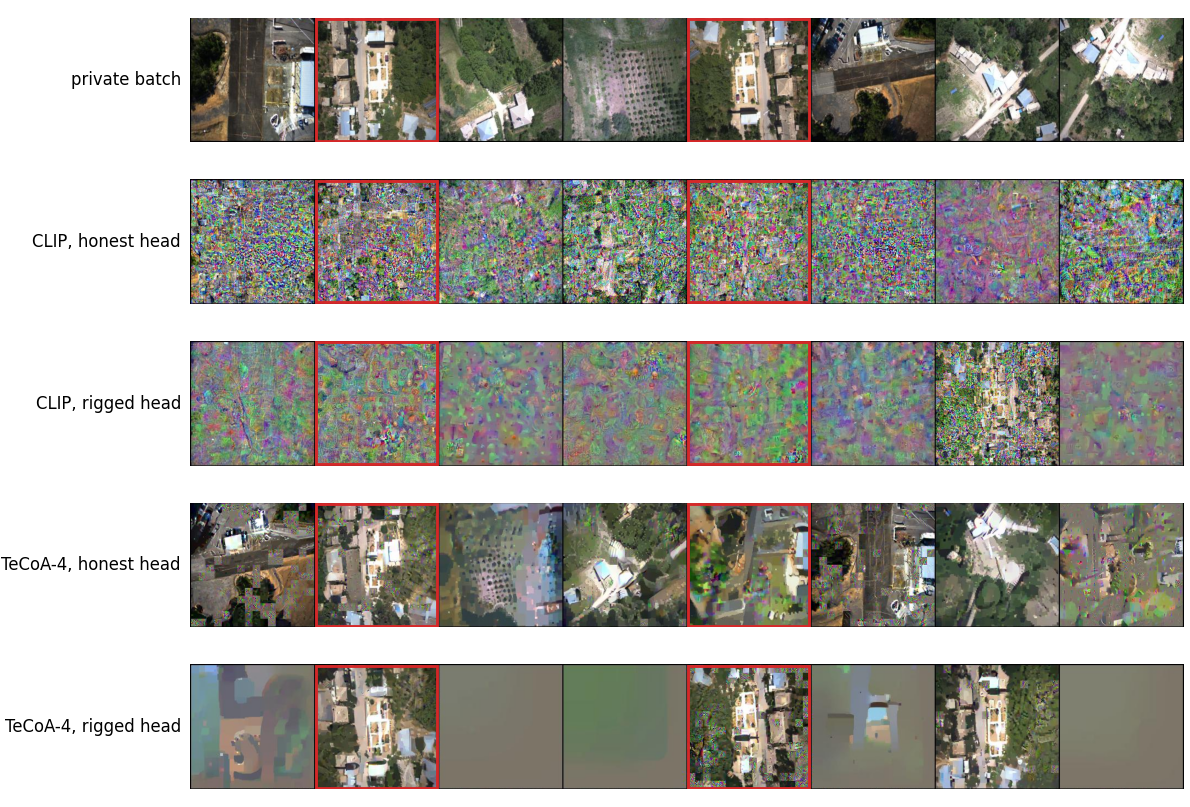
\includegraphics[width=\textwidth]{fig/recon_uav_backbone}
\caption{\textbf{Selection and invertibility are separate factors.} Top row: a client's private batch of eight drone frames, two of which (red) show the rooftop solar panels the attacker asked for. Below: HF-GradInv reconstructions from one shared gradient when the client model is built on vanilla CLIP or on the adversarially fine-tuned TeCoA-4 encoder, each under an honest classifier head and under the head \geminio rigs for the query. The honest head on TeCoA-4 reconstructs the whole batch moderately; the rigged head on TeCoA-4 reconstructs the two targets sharply and sacrifices the rest; on vanilla CLIP neither head recovers anything. Same seed throughout.}
\label{fig:teaser}
\end{figure*}

Federated learning (FL) is sold to hospitals and to operators of camera-equipped drones as a way to train a shared model without ever pooling the images.
Gradient inversion attacks undercut that promise: an honest-but-curious server can optimize dummy inputs until their gradients match the ones a client sent and so recover the client's training images~\cite{dlg2019,ig2020,gradinversion2021}.
A \emph{malicious} server can do better, because it also chooses the model the clients compute gradients on~\cite{robbing2022,fishing2023,garov2024seer}.
\geminio~\cite{geminio2024} is the most targeted attack in this family.
The server writes down what it wants in natural language (``any chest X-ray showing pneumonia''), scores a pool of unlabeled auxiliary images against that query with a vision-language model (VLM), and trains the classifier head it distributes so that images the VLM ranks highly incur a large loss.
When an honest client trains on a private batch, the query-matched images dominate the shared gradient, and an off-the-shelf reconstruction algorithm recovers them.

This paper asks a plain question about that attack: what decides whether it recovers the images it was asked for?
Two ingredients are in play, and prior work has studied them separately.
Malicious-server attacks concentrate the gradient on a few samples~\cite{fishing2023,robbing2022}; adversarially trained models leak more under gradient inversion because their features are easier to invert~\cite{zhang2022privacyat,mejia2019robustorprivate,torp2026nonrobust}.
Adversarially fine-tuned CLIP encoders (TeCoA~\cite{tecoa2023}, FARE~\cite{fare2024}, Sim-CLIP~\cite{simclip2024}) are now the standard way to harden vision-language models, and they can enter the \geminio pipeline in two places: as the attacker's guide, and as the backbone of the client model whose gradient is inverted.
We treat the attack as the product of two factors, \emph{selection}, the share of the client's gradient that the rigged head places on the query-matched images, and \emph{invertibility}, how well the client backbone's features reconstruct, and we measure both directly rather than inferring them from reconstruction quality.

\paragraph{Findings.}
We evaluate \geminio on chest X-rays (ChestMNIST), colorectal histology (PathMNIST) and aerial drone imagery (UAVScenes), with eight guiding VLMs, a ResNet-18 client and ten ViT-L client backbones, three reconstruction algorithms and three seeds per condition, on held-out private batches the rigged heads never saw.
\begin{enumerate}
\itemsep0pt
\item \textbf{Selection tracks the guide's retrieval.} For each of 25 attacker configurations we compute the two target images' share of the summed per-example last-layer weight-gradient norms on the private batch. It is rank-correlated with how well the guide ranks the target class on the auxiliary set (Spearman $\rho=0.67$ over 25 heads; $p=.001$ under a dataset-stratified permutation null). Where the guide ranks the class well the rigged head puts more of that norm on the targets than an honest head does, and on ChestMNIST, where no guide ranks \pneu above 0.64 AUROC, it puts less; no configuration in the project reconstructs a chest X-ray more closely than eight images drawn at random from the dataset (\cref{sec:selection}).
\item \textbf{Robust client backbones reveal what the head selects.} With the query-matched images selected, adversarially fine-tuned ViT-L backbones leak them more than vanilla CLIP (6 of 6, ordered by robustness level) and more selectively; an honest head on the same encoders gives no selectivity, and rigging the head for a different class moves the selectivity to that class. \TODO{comparators: LAION-2B CLIP, DINOv2, supervised IN-21k ViT-L; queue running} (\cref{sec:backbone}).
\item \textbf{Robust guides change reconstruction quality, not selection.} As the attacker's guide, every robust CLIP makes the ChestMNIST attack reconstruct the batch better than vanilla CLIP (18 of 18 seed pairs), yet none of their heads places more than the uniform share of the gradient on the \pneu images. \TODO{PathMNIST guide table, queue running} (\cref{sec:guide}).
\item \textbf{Defense and failure cases.} Noisy, clipped per-update aggregation (\nbfu) removes the drone-imagery reconstruction that the Inverting Gradients attack achieves and weakens \geminio across a 24-query language sweep; clipping alone does nothing. Indirect and terse queries break the attack, misspelled, translated and negated queries do not, and retrieval failure is its dominant failure mode (\cref{sec:failure,sec:defense}).
\end{enumerate}
Along the way we correct two practices from the \geminio evaluation protocol that hid these results: the attack-F1 metric, which scores pure-noise reconstructions near 1.0, and the absence of a reference for what an uninformative reconstruction scores, which we supply with random draws from the dataset scored through the same matching code.

% CVPR 2027 related work. Citation keys are in ../custom.bib; entries added
% 2026-10-13 were checked against arXiv, Crossref and proceedings pages.
\section{Related Work}
\label{sec:related}

\paragraph{Gradient inversion attacks.}
Gradient inversion attacks (GIAs) reconstruct a client's training data by optimizing dummy inputs until their gradients match the ones the client shared.
DLG~\cite{dlg2019} and iDLG~\cite{idlg2020} established the threat, IG~\cite{ig2020} scaled it to ImageNet with cosine matching and a total-variation prior, and GradInversion~\cite{gradinversion2021,deepinversion2020} added BatchNorm-statistic priors for batch recovery; HF-GradInv~\cite{hfgradinv2024}, which Geminio uses for its reconstruction step, extends this line.
Later attacks lean on stronger priors, including pretrained generators (GIFD~\cite{fang2023gifd}), learned denoisers (GUIDE~\cite{guide2025}), style transfer (GI-SMN~\cite{gismn2024}) and searched architectures (GI-NAS~\cite{ginas2025}), and attacks now reach multimodal models~\cite{mmgia2025,gidqa2025}.
A recent survey organizes this literature~\cite{guo2026survey}, while Valadi~\etal~\cite{valadi2025feasibility} argue that optimization-based inversion against an honest server rarely succeeds in production-like training, for example with BatchNorm in training mode.
This makes the actively malicious server, which can shape the model it distributes, the more pressing threat.

\paragraph{Malicious-server attacks.}
An active server can modify the global model so that client updates leak more.
Robbing the Fed~\cite{robbing2022} inserts an imprint layer whose gradients contain individual inputs, Fishing~\cite{fishing2023} rescales output-layer weights so that one target dominates the update, SEER~\cite{garov2024seer} hides the stolen data behind a secret decoder, and ARES~\cite{ares2026} recovers large batches through activation recovery without changing the architecture.
PEFTLeak~\cite{sami2025peftleak} poisons a pretrained ViT backbone once and recovers batches from adapter gradients, which is the threat model closest to our client-side experiments.
VGIA~\cite{vgia2026} adds a test that certifies when a reconstruction is exact.
The same threat now reaches fine-tuning of foundation models, where poisoned pretrained weights or adapters turn LoRA updates into a leakage channel~\cite{minegrad2026,neuroimprint2026}, and recovered client data can be reused to plant backdoors~\cite{aggregatorcheats2026}.
Geminio~\cite{geminio2024} is the first attack in this family to choose targets with natural language: a vision-language model scores the server's auxiliary images against a text query, and the server trains a classifier head that gives matching images a high loss.
We study both how robust vision-language models change this attack and where it fails.

\paragraph{Defenses.}
Differential privacy is the standard formal defense: DP-SGD~\cite{dpsgd2016} clips and noises per-example gradients, and client-level DP~\cite{mcmahan2018learning} protects whole clients.
Work on clipping in federated learning studies convergence and threshold choice~\cite{zhang2021clipping,andrew2021adaptive,dpsfl2024}, and calibrated DP-SGD is known to reduce inversion success~\cite{dp_gia_eval2025}.
Clipping and noise do not stop every attack, however: You~\etal~\cite{you2025ldp} reconstruct samples from updates protected by local DP, and privacy backdoors planted in adapters are reported to evade local DP and clipping, which motivates dedicated defenses~\cite{trishield2026}.
Other defenses detect tampered global models on the client~\cite{carletti2026detect}, augment client data to break active reconstruction~\cite{oasis2026}, project or perturb gradients without a privacy budget~\cite{svdefense2025,cvb2023,tip2026}, aim noise at the image regions an interpretable shadow model marks as sensitive, evaluated on chest X-rays~\cite{shadow2025}, or prune the visual tokens a vision-language model transmits~\cite{qprivvl2026}.
Geminio's authors tested gradient pruning, additive noise and client-side inspection and found them insufficient~\cite{geminio2024}; they did not evaluate clipping, although per-example clipping is known to blunt other malicious-server attacks at a utility cost~\cite{garov2024seer}.

\paragraph{Robust vision-language models and privacy.}
Adversarial fine-tuning hardens CLIP's vision encoder against perturbed inputs, through supervised (TeCoA~\cite{tecoa2023}), unsupervised (FARE~\cite{fare2024}), Siamese (Sim-CLIP~\cite{simclip2024}) and dual-level contrastive (SLADE~\cite{slade2025}) objectives; LEAF~\cite{leaf2025} extends robustness to the text encoder.
Robustness and privacy are known to pull against each other in classifiers.
Adversarially trained models are more exposed to membership inference~\cite{song2019privacy}, are easier to invert~\cite{mejia2019robustorprivate}, and have input gradients and representations that align with human perception~\cite{tsipras2019,santurkar2019,engstrom2019robustprior}.
Recent work makes the tradeoff explicit: model-inversion leakage tracks adversarial robustness across defenses~\cite{torp2026nonrobust,smith2026adaptivemi}, to the point that deliberately learning non-robust features is proposed as a reconstruction defense~\cite{torp2026nonrobust}.
Closest to our setting, Zhang~\etal~\cite{zhang2022privacyat} show that federated clients performing adversarial training leak more under gradient inversion, and LeakyCLIP~\cite{chen2026leakyclip} uses adversarial fine-tuning to make CLIP embeddings easier to invert.
Zhang~\etal\ attribute the extra leakage to adversarial training lowering the probability assigned to the ground-truth class: the output-layer weight gradient for that class is then approximately $-(1-p_{i,y_i})\,r_i$, a scaled copy of the sample's feature vector, which their attack recovers with a scale-invariant cosine objective. Geminio's loss amplification lowers the same probability on clean inputs, for the query-matched samples only.
To our knowledge, no prior work examines robust CLIP encoders in a language-guided attack, either as the attacker's guide or as the backbone of the client model, or tests how these two ingredients combine.

% Background and threat model. Mechanism statement follows Zhang, Chen & Li (CVPRW 2022) as corrected 2026-10-31
% (scaled copy, not clean copy); see results/complementarity/validation_2026_10_27_checks.md.
\section{Background and Threat Model}
\label{sec:background}

\paragraph{Federated learning and gradient inversion.}
We consider FedSGD: in each round the server sends model parameters $\theta$ to a client, which computes the mean gradient $g=\frac{1}{B}\sum_{i=1}^{B}\nabla_\theta \ell(f_\theta(x_i),y_i)$ over a private batch of $B$ images and returns it.
A gradient inversion attack recovers the batch by optimizing dummy inputs $\hat{x}$ so that their gradient matches $g$ under a distance such as the cosine objective of Inverting Gradients (IG)~\cite{ig2020}, with image priors added by GradInversion~\cite{gradinversion2021} and the layer-weighted schedule of HF-GradInv~\cite{hfgradinv2024}, which \geminio uses.
We run the same three algorithms and report HF-GradInv unless stated.

\paragraph{\geminio.}
The server is malicious but passive in the protocol: it sends an honest-looking model and reads honest gradients.
Before the round it holds a pool of unlabeled auxiliary images $\{a_j\}$, a text query $q$ and a VLM with image and text encoders $E_I,E_T$.
It trains only the classifier head $h_\phi$ on frozen backbone features so that images the VLM ranks as similar to $q$ incur a large loss~\cite{geminio2024}:
\begin{equation}
\min_\phi \; \mathbb{E}_{\text{batch}}\Big[\textstyle\sum_j \tilde{\ell}_j\,(1-p_j)\Big],\qquad
p_j=\frac{\exp(T\,\langle E_I(a_j),E_T(q)\rangle)}{\sum_{k}\exp(T\,\langle E_I(a_k),E_T(q)\rangle)},
\label{eq:geminio}
\end{equation}
where $\tilde{\ell}_j$ is the per-sample loss normalized within the batch and $T=100$.
The rigged head is distributed as the global model.
We call the VLM the \emph{guide} and $h_\phi$ the \emph{rigged head}; an \emph{honest head} is the same architecture trained with the ordinary mean loss.
The quantity \geminio's authors report, the \emph{loss ratio}, is the mean loss of the top 10\% query-similar auxiliary images over the rest.

\paragraph{Why a rigged head leaks.}
For a cross-entropy head the gradient of the last layer's weights contributed by sample $i$ is $(p_i-y_i)\otimes r_i$, the outer product of the output residual and the penultimate activation $r_i$.
Zhang \etal~\cite{zhang2022privacyat} use this identity to explain why adversarially trained FL clients leak more: training lowers the probability $p_{i,y_i}$ assigned to the true class, so the row for class $y_i$ is approximately $-(1-p_{i,y_i})\,r_i$, a scaled copy of the sample's feature vector that a scale-invariant objective recovers.
\geminio's loss amplification produces the same condition on clean inputs, and only for the samples the guide matched.
Whether a target image is reconstructed therefore depends on two things that can be measured separately on the private batch: how much of the gradient the head places on that image, and how well the backbone's features $r_i$ invert.

\paragraph{Robust CLIP encoders.}
TeCoA~\cite{tecoa2023}, FARE~\cite{fare2024} and Sim-CLIP~\cite{simclip2024} fine-tune the CLIP ViT-L/14 vision tower against $\ell_\infty$ perturbations of radius $\epsilon\in\{2,4\}/255$ with supervised, unsupervised and Siamese objectives respectively, leaving the text encoder unchanged.
We use the six public checkpoints and vanilla OpenAI CLIP~\cite{clip2021}, and add three ViT-L encoders that were never adversarially trained, CLIP trained on LAION-2B~\cite{openclip2023}, DINOv2~\cite{dinov2} and a supervised ImageNet-21k ViT-L/16~\cite{augreg2022}, so that ``robust'' is compared against more than one non-robust checkpoint.
For chest X-rays and histology the domain guide is BiomedCLIP~\cite{biomedclip2023}.

\paragraph{Threat model.}
The client is honest and trains a frozen ImageNet backbone (ResNet-18, or one of the ViT-L encoders above) with a three-layer head on batches of $B=8$ images, two of which match the query; the server knows the labels, as in \geminio.
The attacker observes one gradient and may choose the head, the guide and the query, but not the client's data or backbone.

% Experimental setup. Sources: results/heldout_rerun/summary.md (348 runs), results/client_encoder/summary.md (48),
% results/client_encoder_plain, results/client_encoder_swap_qair_qeff, results/pathmnist/README.md,
% results/complementarity/floor_baselines.md, assets/*_manifest.json.
\section{Experimental Setup}
\label{sec:setup}

\paragraph{Datasets and queries.}
ChestMNIST (64\,px chest X-rays, 14 findings plus ``normal'', 22{,}433 test images)~\cite{medmnistv2} with the query ``any chest X-ray showing pneumonia'';
PathMNIST (64\,px colorectal histology, 9 tissue classes, 7{,}180 test images)~\cite{medmnistv2} with the query ``any colorectal histopathology image showing colorectal adenocarcinoma epithelium'';
and UAVScenes (drone frames from two scenes with 18 semantic classes)~\cite{uavscenes2024} with the query ``aerial drone image showing solar panels on rooftops''.
In each dataset the first half of every class is the attacker's auxiliary pool and the second half is held out; private batches are drawn from the held-out half only and contain two target images among eight, with the six others from distinct classes.
The PathMNIST target class was fixed from a retrieval scan of all nine classes under all eight guides before any attack ran: it is the clinically sensitive class, and the guides spread from 0.54 to 0.87 AUROC on it.

\paragraph{Attacker configurations.}
Guides: BiomedCLIP for the two medical datasets, vanilla CLIP for UAV, and the six robust CLIPs in every dataset (eight guides for medical, seven for UAV).
Client models: a ResNet-18 with the \geminio head (512$\to$256$\to$64$\to$C), and the ten ViT-L encoders of \cref{sec:background} with the same head on their pooled features (inputs stay ImageNet-normalized and are re-normalized inside the model).
Rigged heads are trained on cached backbone features for 5 epochs with Adam ($10^{-3}$), $T=100$, batch 16, seed 0; honest heads identically with the mean loss; swapped-query heads with a second query of a class present in the batch (pleural effusion; airport runway).
Reconstruction: HF-GradInv for 24{,}000 iterations with its layer window scaled to each architecture's parameter count, plus IG and GradInversion for the defense comparison; seeds 42, 123 and 256 per condition.
BatchNorm runs in evaluation mode with the public running statistics, the \geminio default; the training-mode variant is reported as a robustness check.

\paragraph{Metrics.}
\geminio's attack F1 counts a reconstruction as a hit when its last-layer gradient has cosine similarity above 0.9 with the true one; with the true label fed to both sides it scores pure-noise reconstructions at 1.0, so we do not use it.
We report \emph{target \lpips}, the \lpips distance~\cite{lpips2018} between each target image and its best-matching reconstruction (lower is more leakage), the same for non-targets, and \emph{selectivity}, non-target minus target \lpips (positive when the targets come out better).
Because best-match lets several images share one reconstruction (it does so in 37\% of runs), every table also carries the one-to-one Hungarian assignment that minimizes total \lpips.
\emph{Target share} is the two target images' fraction of the summed per-example last-layer weight-gradient norms, $\|p_i-y_i\|\,\|r_i\|$; equal contribution is 0.25. It allocates a sum of per-example norms, which is not the norm of the transmitted sum, and it covers the head's last layer while the shared gradient spans the whole model, so we use it alongside the paired contrast against an honest head rather than as an absolute measure of what the attacker sees.
\emph{Reference values}: eight images drawn at random from the auxiliary half and scored through the same matching code, 50 draws per batch, give the target \lpips and selectivity an uninformative reconstruction obtains (ChestMNIST 0.327 [5th--95th percentile 0.294, 0.361]; PathMNIST 0.420 [0.383, 0.451]; UAV 0.535 [0.485, 0.571]). Only values below the 5th percentile evidence recovery; paired contrasts are unaffected, because the reference depends only on the batch.

\paragraph{Statistics.}
Conditions are compared seed by seed with paired $t$-tests ($n=3$, $df=2$) and, across encoders or queries, with Wilcoxon signed-rank tests whose floor at seven encoders is $p=.016$.
We state as findings only effects that survive Holm correction within their table or hold on every seed pair; everything else is given with its direction and $n$.
Every condition uses one private batch per dataset, so the seeds vary the reconstruction optimizer, not the data; we flag this in \cref{sec:discussion}.

% Results. Sources per subsection are given in the comments. \TODO marks numbers still pending from the Nov 2 queue
% (results/nov-runs/*): PathMNIST attacks and the three non-robust comparator encoders.
\section{Results}
\label{sec:results}

\subsection{Selection is bounded by retrieval}
\label{sec:selection}
% results/complementarity/retrieval_vs_selection.md, private_batch_profile_resnet18.md, private_batch_profile.md,
% vlm_retrieval.md, results/pathmnist/retrieval_scan.md, floor_baselines.md, baseline_comparison.md

\begin{figure}[t]
\centering
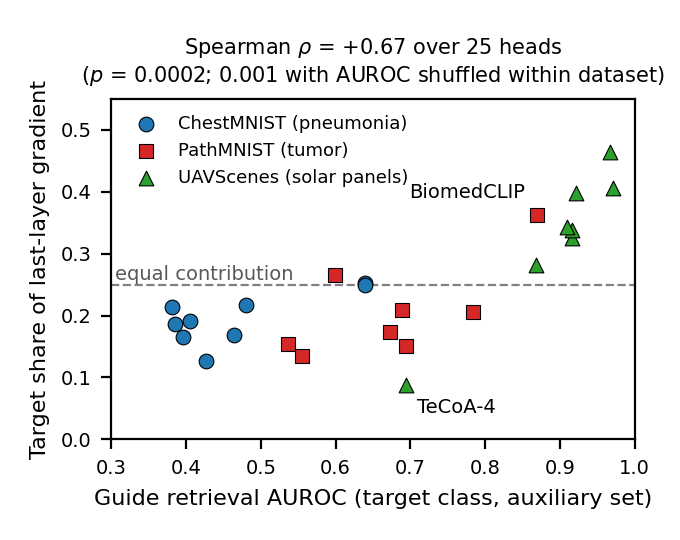
\includegraphics[width=\linewidth]{fig/retrieval_vs_share}
\caption{\textbf{The rigged head selects its targets only when the guide retrieves them.} One point per guide head (ResNet-18 client, 25 heads over three datasets): the AUROC with which the guide's query similarity ranks the target class on the attacker's auxiliary set, against the share of the client's last-layer gradient that the two target images of the private batch receive. Uniform share is 0.25. ChestMNIST guides all sit below 0.65 AUROC and no head selects; the one UAV guide that fails retrieval (TeCoA-4) is the one UAV head that does not select.}
\label{fig:retrieval}
\end{figure}

\begin{table}[t]
\centering
\small
\caption{\textbf{What the rigged head does to the private batch.} For each dataset and guide, the share of the client's last-layer gradient norm that the two target images receive (uniform $=0.25$), the head's mean loss on the targets over its loss on the other six images, and the guide's retrieval AUROC for the target class on the auxiliary set. ResNet-18 client, held-out batch, one head per guide.}
\label{tab:profile}
\begin{tabular}{llccc}
\toprule
Dataset & Guide & AUROC & Target share & Loss ratio \\
\midrule
\multirow{4}{*}{ChestMNIST} & BiomedCLIP & 0.64 & 0.249 & 2.4$\times$ \\
 & CLIP & 0.48 & 0.216 & 0.8$\times$ \\
 & best robust (FARE-2) & 0.38 & 0.214 & 0.9$\times$ \\
 & worst robust (TeCoA-2) & 0.43 & 0.127 & 0.5$\times$ \\
\midrule
\multirow{4}{*}{PathMNIST} & BiomedCLIP & 0.87 & \textbf{0.362} & 1.9$\times$ \\
 & CLIP & 0.60 & 0.266 & 0.4$\times$ \\
 & TeCoA-4 & 0.78 & 0.205 & 0.2$\times$ \\
 & SimCLIP-2 & 0.56 & 0.135 & 0.2$\times$ \\
\midrule
\multirow{4}{*}{UAVScenes} & CLIP & 0.92 & \textbf{0.338} & 2.1$\times$ \\
 & SimCLIP-2 & 0.97 & \textbf{0.464} & 9.5$\times$ \\
 & FARE-2 & 0.97 & \textbf{0.406} & 9.3$\times$ \\
 & TeCoA-4 & 0.69 & 0.087 & 0.02$\times$ \\
\bottomrule
\end{tabular}
\end{table}

\geminio's own diagnostic, the loss ratio on the auxiliary set, says that every head we trained is rigged: 8--14$\times$ on ChestMNIST, 17--28$\times$ on PathMNIST, 19--131$\times$ on UAV.
The private batch tells a different story (\cref{tab:profile}; full table in the supplement).
On UAV, seven of eight guide heads place more than the uniform share of the last-layer gradient on the two solar-panel images (0.28--0.46), with the targets' own-label probability driven down to 0.22--0.39 against 0.48--0.80 for the rest.
The exception is TeCoA-4, the one UAV guide whose query similarity fails to rank solar panels (AUROC 0.69 against 0.87--0.97 for the others): its head puts 0.087 of the gradient on the targets and makes them the \emph{easiest} images in the batch.
On ChestMNIST no head exceeds the uniform share. The BiomedCLIP heads sit exactly at it (0.249, 0.253); every CLIP-family head is below it (0.13--0.22), and the robust-guide heads reach per-image losses of 250--860 on every image of the batch, targets and non-targets alike.
On PathMNIST only the BiomedCLIP head, the one guide with AUROC above 0.75, selects the tumor images (0.362); the seven CLIP-family heads, with AUROC 0.54--0.78, place 0.13--0.27 on them.

Across the 25 heads the target share follows retrieval: Spearman $\rho=0.67$ ($p=.0002$); within UAV, $\rho=0.90$.
Split at 0.75 AUROC, 8 of 9 heads above the threshold select their targets (median share 0.34) and 2 of 16 below it do (median 0.18).
The same holds for the ViT-L client, where the rigged head puts 0.52 of the gradient on the UAV targets (7 of 7 encoders) but 0.15 on the \pneu images, below the uniform share and below its own honest head (0.29).

This resolves the medical result end to end. Vanilla CLIP and all six robust CLIPs rank \pneu at or below chance on the ChestMNIST auxiliary set (any-label AUROC 0.42--0.49, base rate 1.2\%), and the top-ranked auxiliary images under every guide are mostly ``normal'' radiographs no closer in \lpips to the held-out targets than random ones.
A head trained by \cref{eq:geminio} to amplify whatever the guide scores highly therefore learns to amplify a non-\pneu subset, and on the private batch the \pneu images receive no amplification.
Reconstruction then has nothing to select: no ChestMNIST configuration in this study, across two client architectures, 24 queries, eight guides and three reconstruction algorithms, reaches a target \lpips below the 95th percentile of eight random draws from the dataset (best 0.377 against a reference of 0.327 [0.294, 0.361]).
Part of this is the metric, since 64\,px radiographs upscaled to 224\,px are mutually similar under \lpips; the selection failure is not, and it is measured before any reconstruction runs.
\TODO{PathMNIST: does the BiomedCLIP head's 0.36 share turn into selectivity above the reference and target \lpips below it? Group A, Nov 2.}

\subsection{Robust client backbones reveal what the head selects}
\label{sec:backbone}
% results/client_encoder/summary.md, results/client_encoder_plain/summary.md, results/client_encoder_swap_qair_qeff/summary.md,
% results/plain_head/README.md (limits), results/complementarity/private_batch_profile.md

\begin{figure*}[t]
\centering
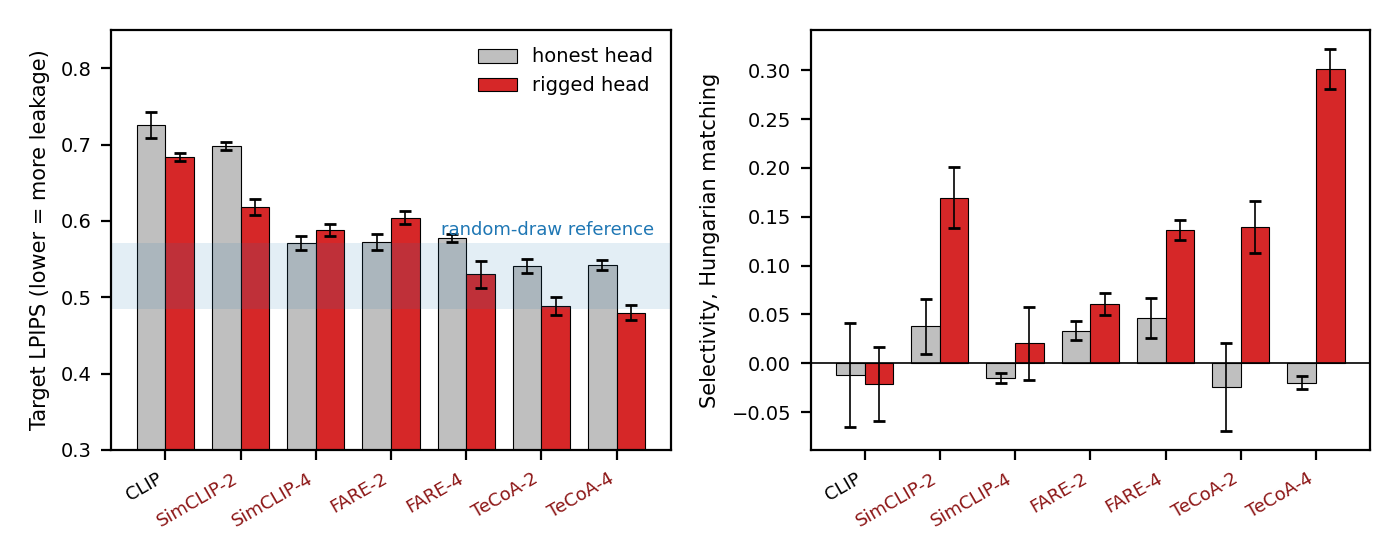
\includegraphics[width=\textwidth]{fig/backbone_uav}
\caption{\textbf{Client backbone and head type on UAV.} Target \lpips (left; shaded band is the 5th--95th percentile of the random-draw reference) and Hungarian selectivity (right) for each ViT-L client encoder under an honest head and under the head rigged for solar panels; mean and standard error over three seeds. Robust encoders in red on the axis. The honest head is never selective; the rigged head is selective only on robust encoders, increasingly with robustness level. \TODO{add the three non-robust comparators when their runs finish.}}
\label{fig:backbone}
\end{figure*}

\begin{table}[t]
\centering
\small
\caption{\textbf{Client backbone, UAV solar-panel targets.} Target \lpips (lower is more leakage) and selectivity (non-target minus target \lpips) under the rigged head and under an honest head on the same frozen encoder, mean over three seeds; $\Delta$ is paired against vanilla CLIP under the rigged head. Hungarian selectivity in parentheses. The bottom block adds encoders that were never adversarially trained. \TODO{comparator rows from results/nov-runs}}
\label{tab:backbone}
\begin{tabular}{lcccc}
\toprule
 & \multicolumn{2}{c}{Rigged head} & \multicolumn{2}{c}{Honest head} \\
\cmidrule(lr){2-3}\cmidrule(lr){4-5}
Encoder & Target \lpips & Selectivity & Target \lpips & Selectivity \\
\midrule
CLIP (OpenAI) & 0.683 & $-$0.007 ($-$0.02) & 0.726 & $-$0.000 \\
SimCLIP-2 & 0.618 & +0.036 (+0.17) & 0.698 & +0.02 \\
SimCLIP-4 & 0.589 & +0.025 (+0.02) & 0.571 & $-$0.01 \\
FARE-2 & 0.604 & +0.032 (+0.06) & 0.572 & +0.01 \\
FARE-4 & 0.530 & +0.067 (+0.14) & 0.578 & $-$0.01 \\
TeCoA-2 & 0.489 & +0.092 (+0.14) & 0.541 & $-$0.00 \\
TeCoA-4 & \textbf{0.480} & \textbf{+0.122} (+0.30) & 0.542 & +0.01 \\
\midrule
CLIP (LAION-2B) & \TODO{} & & & \\
DINOv2 & \TODO{} & & & \\
ViT-L/16 IN-21k & \TODO{} & & & \\
\midrule
ResNet-18 & 0.476 & +0.114 (+0.20) & -- & -- \\
\bottomrule
\end{tabular}
\end{table}

On UAV, where the head selects, all six adversarially fine-tuned ViT-L backbones leak the targets more than vanilla CLIP (paired $p\le.019$, 6 of 6), the effect is ordered by robustness level within each family ($\epsilon=4$ leaks more than $\epsilon=2$), and the gain on the query-matched images is 1.5--3 times the gain on the rest, so selectivity rises from zero to +0.12 (+0.30 under one-to-one matching) on TeCoA-4 (\cref{tab:backbone}).
Only TeCoA-4's target \lpips (0.480) falls below the 5th percentile of the random-draw reference (0.485); the rest of the robust encoders sit inside or above it.

Three controls separate the two factors.
\emph{Honest head}: trained with the mean loss on the same frozen encoders, it gives selectivity within $\pm0.02$ on all seven encoders, and the paired drop from the rigged head is significant on 5 of 7 (Wilcoxon over encoders $p=.031$).
Yet the honest head still reconstructs robust encoders' batches better than CLIP's (target \lpips 0.54--0.70 against 0.73; 5 of 6 encoders, $p\le.02$): invertibility is a property of the backbone that exists without rigging, and the rigged head adds only +0.03 target \lpips on top of it.
\emph{Swapped query}: rigging the head for airport runways instead of solar panels on the same batch removes the solar selectivity (6 of 7 encoders, $p=.031$) and raises solar target \lpips on 7 of 7 while leaving non-targets unchanged; the selectivity is a property of the query, not of rigging in general.
\emph{Gradient share}: the rigged head puts 0.52 of the last-layer gradient on the two targets (0.37--0.69 across the seven encoders), the honest head 0.15 and the runway head 0.10, with the runway images then taking 0.28--0.66.
Low confidence on the matched images and a concentrated gradient appear together, and only under the head rigged for them.

Two things these controls do not show.
The ``interaction'' between head and backbone, positive on all six robust encoders, is measured against a single non-robust comparator, so the bottom block of \cref{tab:backbone} adds three ViT-L encoders that were trained without adversarial fine-tuning. \TODO{state what they show: if LAION-2B CLIP, DINOv2 and the supervised ViT-L invert as well as the robust CLIPs, the effect is about the encoder family rather than robustness; if not, it is specific to adversarial fine-tuning.}
And on ChestMNIST every ViT-L client fails regardless of robustness (target \lpips 0.76--0.87; honest head 0.67--0.87), which \cref{sec:selection} attributes to the head never selecting the targets rather than to the backbone.

\subsection{Robust guides change reconstruction quality, not selection}
\label{sec:guide}
% results/heldout_rerun/summary.md block 2 (medical_vlm*_ho, uav_vlm*_ho), results/complementarity/vlm_retrieval.md,
% aux_appearance.md; PathMNIST guide table pending (results/nov-runs/pathmnist-resnet)

\begin{table}[t]
\centering
\small
\caption{\textbf{Guide VLM, ResNet-18 client.} Target \lpips, mean over three seeds, with the paired difference against vanilla CLIP as the guide; negative means a stronger attack. BiomedCLIP is the domain guide for the medical datasets. \TODO{PathMNIST column from results/nov-runs/pathmnist-resnet}}
\label{tab:guide}
\begin{tabular}{lcccccc}
\toprule
 & \multicolumn{2}{c}{ChestMNIST} & \multicolumn{2}{c}{PathMNIST} & \multicolumn{2}{c}{UAVScenes} \\
\cmidrule(lr){2-3}\cmidrule(lr){4-5}\cmidrule(lr){6-7}
Guide & \lpips & $\Delta$ & \lpips & $\Delta$ & \lpips & $\Delta$ \\
\midrule
BiomedCLIP & 0.590 & $-$0.10 & \TODO{} & & -- & -- \\
CLIP & 0.687 & -- & & -- & 0.470 & -- \\
SimCLIP-2 & 0.448 & $-$0.24 & & & 0.473 & +0.00 \\
SimCLIP-4 & 0.444 & $-$0.24 & & & 0.565 & +0.10 \\
FARE-2 & \textbf{0.377} & $-$0.31 & & & 0.515 & +0.04 \\
FARE-4 & 0.491 & $-$0.20 & & & 0.562 & +0.09 \\
TeCoA-2 & 0.411 & $-$0.28 & & & 0.496 & +0.03 \\
TeCoA-4 & 0.419 & $-$0.27 & & & 0.591 & +0.12 \\
\bottomrule
\end{tabular}
\end{table}

When a robust CLIP replaces vanilla CLIP as the guide while the client stays a ResNet-18, the ChestMNIST attack reconstructs the batch better on every robust guide (6 of 6, 18 of 18 seed pairs, sign test $p=8\times10^{-6}$; \cref{tab:guide}), and the ImageNet-robust guides beat the domain guide BiomedCLIP as well.
This is not a targeting effect. \Cref{tab:profile} shows that none of these heads places the uniform share of the gradient on the \pneu images, and non-target \lpips improves by as much as target \lpips (selectivity stays within $\pm0.07$ of zero for all guides).
What changes is the loss regime: the robust-guide heads assign per-image losses two orders of magnitude larger than the vanilla-CLIP head to every image in the batch, which makes the whole gradient easier to invert.
On UAV, where retrieval differs by guide, there is no robust-guide effect on average (6 of 18 seed pairs), but retrieval precision tracks attack strength across the seven guides ($\rho=-0.86$, $p=.014$), and the guide that fails retrieval (TeCoA-4) gives the weakest attack.
\TODO{PathMNIST: guide retrieval spreads 0.54--0.87 here, so this is the cleanest test of retrieval against attack strength within one dataset.}

\subsection{Where the attack fails}
\label{sec:failure}
% results/heldout_rerun/summary.md block 3 (24-query sweep) and block 4 (floor conditions); abstract.tex comment (3)

Across 12 query variants per domain (table in the supplement), the ChestMNIST attack is strongest with a misspelled query (target \lpips 0.40) and a purely negated one (0.46), close to the base query (0.51) with a Spanish translation (0.53), and breaks with an exclusion (``not pneumonia'', 0.67), a disjunction (0.70), a terse one-word query (0.71) and an indirect description (0.93).
On UAV every variant lands between 0.44 and 0.54.
Misspelling, translation and negation therefore do not weaken the attack, because the guide's embedding absorbs them; what weakens it is a query whose embedding no longer retrieves the class.
Four further conditions are floors rather than findings: ChestMNIST at batch 32, BatchNorm in training mode, GradInversion on ChestMNIST and the indirect query all leave the undefended attack at target \lpips $\ge0.7$, consistent with Valadi \etal~\cite{valadi2025feasibility}, so no defense result should be read from them.

% Defense. Sources: results/heldout_rerun/summary.md blocks 1, 3 and 4; results/complementarity/baseline_comparison.md;
% prototype/defenses.py (analytic Gaussian calibration, sensitivity 2C).
\section{Defense: Noisy Clipped Updates}
\label{sec:defense}

\geminio's authors report that gradient pruning, additive Laplacian noise and client-side inspection do not stop the attack~\cite{geminio2024}; they did not test clipping with calibrated noise, the mechanism of DP-SGD~\cite{dpsgd2016}.
We evaluate the simplest form of it, \nbfu: the client clips its mean update to $\ell_2$ norm $C=1$ and adds Gaussian noise calibrated by the analytic mechanism~\cite{balle2018analytic} to $(\varepsilon,\delta)=(5,10^{-5})$ with sensitivity $2C$ for the per-update release.
This is per-update aggregate DP, not record-level DP; a record-level variant with per-example clipping gives the same reconstruction numbers.

\begin{table}[t]
\centering
\small
\caption{\textbf{\nbfu at $\varepsilon=5$ against three reconstruction algorithms}, ResNet-18 client, base queries, target \lpips (mean of three seeds) and paired $\Delta$. The reference column is the random-draw value an uninformative reconstruction obtains; only numbers below it show recovery.}
\label{tab:defense}
\begin{tabular}{llcccc}
\toprule
Dataset & Attack & Undefended & \nbfu & $\Delta$ ($p$) & Reference \\
\midrule
\multirow{3}{*}{ChestMNIST} & HF-GradInv & 0.564 & 0.805 & +0.24 (.056) & \multirow{3}{*}{0.33 [0.29, 0.36]} \\
 & IG & 0.592 & 0.822 & +0.23 (.005) & \\
 & GradInversion & 0.922 & floor & -- & \\
\midrule
\multirow{2}{*}{PathMNIST} & HF-GradInv & 0.534 & 0.802 & +0.27 (.013) & \multirow{2}{*}{0.42 [0.38, 0.45]} \\
 & IG & 0.498 & 0.831 & +0.33 (.005) & \\
\midrule
\multirow{3}{*}{UAVScenes} & HF-GradInv & 0.470 & 0.689 & +0.22 (.108) & \multirow{3}{*}{0.54 [0.49, 0.57]} \\
 & IG & \textbf{0.453} & 0.727 & +0.27 (.002) & \\
 & GradInversion & 0.520 & 0.712 & +0.19 & \\
\bottomrule
\end{tabular}
\end{table}

\paragraph{Read against the reference.}
On UAV the undefended IG attack sits below the 5th percentile of the random-draw reference, so its reconstruction carries signal, and \nbfu moves it to 0.727, above the reference: the defense removes a signal that was present (\cref{tab:defense}).
Across the 24-query language sweep, \nbfu raises target \lpips on 12 of 12 UAV queries and 11 of 12 ChestMNIST queries (69 of 72 seed pairs under best-match, 63 of 72 under Hungarian matching), and that block survives Holm correction.
Against HF-GradInv on a single batch the direction is the same in both domains but is not separable from seed noise at $n=3$.
On the two medical datasets the undefended attack is already at or above the reference, so the defended numbers show that nothing was recovered either way, not that the defense stopped a recovery. The PathMNIST contrasts are the largest in the table (+0.27 and +0.33, both significant at $n=3$) and still carry that caveat, which is why we read \cref{tab:defense} by the reference column and not by the size of $\Delta$.

\paragraph{Noise, not clipping.}
Clipping alone ($\sigma=0$) changes target \lpips by 0.03--0.06 in every condition, none significant; the budget sweep from $\varepsilon=0.1$ to $50$ gives the same defended values (0.80 ChestMNIST, 0.69 UAV) and so does the clipping bound from $C=0.1$ to $5$ at fixed $\varepsilon$.
The defense is therefore the calibrated noise; clipping is what makes the noise calibratable.
Claims at batch 16 and 32 depend on which matching is used, and we do not make them.

\paragraph{Cost.}
On these frozen-backbone heads, accuracy is unchanged down to $\varepsilon\approx10$ and drops sharply below $\varepsilon\approx5$ (supplement), so the operating point we test is at the edge of what a client would accept; a multi-round attacker averaging $T$ independent releases shrinks the noise by $\sqrt{T}$, which the supplement quantifies.

% Discussion, limitations, conclusion. Limits follow results/{plain_head,query_swap,temp_sweep,complementarity}/README.md
% "Limits of this control" sections (independent review 2026-10-27).
\section{Discussion}
\label{sec:discussion}

\paragraph{What the two factors buy an attacker and a defender.}
For the attacker, the guide is the bottleneck: \geminio's loss ratio certifies that a head is rigged, not that it is rigged for the right images, and a guide that cannot retrieve the class on the attacker's own auxiliary pool (chest X-rays at 64\,px for every CLIP variant; solar panels for TeCoA-4) produces a head that spends the gradient elsewhere.
Domain guides help when they retrieve (BiomedCLIP on histology) and not otherwise (BiomedCLIP on ChestMNIST, AUROC 0.64).
For the defender, two conclusions follow. First, adversarial robustness in the client backbone is not neutral: with a selecting head it concentrates the leakage on the images the attacker asked for, in proportion to the robustness level. Second, the retrieval failure that protects ChestMNIST here is an accident of resolution and class, not a property of medical imaging, and it should not be relied on.

\paragraph{Robust guides.}
The ChestMNIST guide effect (\cref{sec:guide}) is real and survives correction, but it is a whole-batch effect carried by the loss regime the robust-guide heads land in, not by selection.
We report it because the \geminio protocol would count it as the attack getting stronger, and because a reader of the loss ratio alone would conclude the opposite of what the private batch shows.

\paragraph{Limitations.}
Every condition uses one private batch per dataset; seeds vary the reconstruction optimizer, not the data, so the paired contrasts generalize to other batches only by assumption.
The gradient share is computed for the head's last layer; the full gradient includes the backbone, whose per-sample decomposition we did not measure.
Medical images are 64\,px MedMNIST renderings, which compresses \lpips and is part of why no chest X-ray configuration clears the reference; higher-resolution data may move both the attack and the reference.
Three seeds per condition leave several directionally consistent effects unresolved, and the Wilcoxon tests over seven encoders have a floor of $p=.016$.
The honest-head control removes both query weighting and per-batch loss normalization at once; a uniform-weight head would isolate the weighting.
We did not run generative-prior attacks (GIFD, GUIDE) or the real SLADE checkpoints, whose public weights are copies of Sim-CLIP's.

\section{Conclusion}
\label{sec:conclusion}
Language-guided gradient inversion leaks what its guide can retrieve and what its client backbone can invert.
Measured on the private batch, the rigged head selects its targets only when the guiding VLM ranks the target class well, and adversarially fine-tuned client backbones turn that selection into reconstructions in proportion to their robustness.
Where the guide fails, as it does for pneumonia on 64\,px chest X-rays under every CLIP variant we tested, the attack never selects the targets and recovers nothing a random draw would not; where it succeeds, calibrated noise on clipped updates removes the recovery while clipping alone does not.
We release the pipeline, the held-out batches, the per-sample profiles and the reference baselines so that future language-guided attacks are evaluated against what their heads actually select.

% Mandatory CVPR 2027 section (desk reject if missing): after the main text, before the references.
% TODO(Dan): approve the wording. It names no tool or vendor, in line with the repository policy, and must be true
% of the final submission; adjust if the division of labor changes.
\section*{LLM Usage Statement}
Large language model based assistants were used to draft and refactor analysis code, to generate result tables from the saved run outputs, and to edit prose.
All experiments were designed by the authors, every reported number was recomputed from the saved tensors by scripts in the released repository, and the authors reviewed and take responsibility for all text, claims and code.

{
    \small
    \bibliographystyle{ieeenat_fullname}
    \bibliography{../custom}
}

% Supplementary pages are submitted separately (Nov 23); keep them out of the main PDF.
% % Supplementary material (separate upload, due Nov 23). Build standalone by uncommenting % Supplementary material (separate upload, due Nov 23). Build standalone by uncommenting % Supplementary material (separate upload, due Nov 23). Build standalone by uncommenting \input{sec/X_suppl} in main.tex
% and commenting the other sections. Sources: results/heldout_rerun/summary.md (block 3), prototype/language_sweep_config.py,
% results/complementarity/private_batch_profile_resnet18.md.
\clearpage
\setcounter{page}{1}
\maketitlesupplementary

\section{Language sweep}
\label{sec:suppl_lang}

\begin{table*}[h]
\centering
\small
\caption{\textbf{24-query language sweep}, ResNet-18 client, held-out batches, target \lpips (mean $\pm$ 95\% CI over three seeds) without and with \nbfu at $\varepsilon=5$. Variants are grouped as paraphrase, composition, negation and surface diversity.}
\label{tab:lang}
\begin{tabular}{llcc}
\toprule
Dataset & Query & Undefended & \nbfu $\varepsilon=5$ \\
\midrule
\multirow{12}{*}{ChestMNIST}
 & Any chest X-ray showing pneumonia (base) & 0.513 $\pm$ 0.050 & 0.825 $\pm$ 0.008 \\
 & pneumonia (terse) & 0.713 $\pm$ 0.143 & 0.785 $\pm$ 0.024 \\
 & A frontal chest radiograph demonstrating airspace consolidation consistent with pneumonia & 0.573 $\pm$ 0.070 & 0.781 $\pm$ 0.041 \\
 & Chest imaging revealing signs of bacterial pneumonia & 0.490 $\pm$ 0.033 & 0.828 $\pm$ 0.004 \\
 & Lung infection visible on chest radiograph (indirect) & 0.930 $\pm$ 0.070 & 0.816 $\pm$ 0.045 \\
 & Any chest X-ray showing pneumonia and cardiomegaly & 0.497 $\pm$ 0.091 & 0.871 $\pm$ 0.092 \\
 & Any chest X-ray showing either pneumonia or pleural effusion & 0.699 $\pm$ 0.203 & 0.831 $\pm$ 0.030 \\
 & Any chest X-ray showing pneumonia without pleural effusion & 0.672 $\pm$ 0.091 & 0.823 $\pm$ 0.008 \\
 & Any chest X-ray that does not show pneumonia & 0.462 $\pm$ 0.071 & 0.807 $\pm$ 0.009 \\
 & Cualquier radiografia de torax que muestre neumonia & 0.526 $\pm$ 0.071 & 0.820 $\pm$ 0.039 \\
 & Any chst Xray showing pneumon (typo) & 0.398 $\pm$ 0.040 & 0.824 $\pm$ 0.025 \\
 & 30-word clinical description (long) & 0.485 $\pm$ 0.189 & 0.785 $\pm$ 0.033 \\
\midrule
\multirow{12}{*}{UAVScenes}
 & aerial drone image showing solar panels on rooftops (base) & 0.509 $\pm$ 0.064 & 0.684 $\pm$ 0.036 \\
 & solar panels (terse) & 0.457 $\pm$ 0.185 & 0.685 $\pm$ 0.016 \\
 & high-altitude aerial photograph capturing photovoltaic panel installations atop rooftops & 0.537 $\pm$ 0.044 & 0.676 $\pm$ 0.039 \\
 & drone view of rooftop photovoltaic installations & 0.541 $\pm$ 0.049 & 0.685 $\pm$ 0.016 \\
 & Solar power infrastructure visible from above (indirect) & 0.510 $\pm$ 0.203 & 0.675 $\pm$ 0.036 \\
 & aerial drone image showing solar panels on residential rooftops in a suburban neighborhood & 0.527 $\pm$ 0.037 & 0.688 $\pm$ 0.042 \\
 & aerial drone image showing either solar panels or wind turbines & 0.544 $\pm$ 0.037 & 0.691 $\pm$ 0.057 \\
 & aerial drone image showing solar panels without trees blocking the view & 0.510 $\pm$ 0.134 & 0.683 $\pm$ 0.050 \\
 & aerial drone image that does not show solar panels & 0.441 $\pm$ 0.231 & 0.692 $\pm$ 0.026 \\
 & Imagen aerea de dron mostrando paneles solares en tejados & 0.533 $\pm$ 0.067 & 0.695 $\pm$ 0.012 \\
 & aerial dron image showing solar panles on rofotops (typo) & 0.493 $\pm$ 0.096 & 0.682 $\pm$ 0.023 \\
 & 40-word description from a quadcopter at altitude (long) & 0.462 $\pm$ 0.153 & 0.678 $\pm$ 0.017 \\
\bottomrule
\end{tabular}
\end{table*}

\section{Per-sample profile of every guide head}
\label{sec:suppl_profile}
Full version of \cref{tab:profile}: for every (dataset, guide) pair, the guide's retrieval AUROC for the target class on the auxiliary set, the target share of the last-layer gradient (bold when above the uniform 0.25), the mean probability the head assigns to the own label of the targets and of the other six images, and the mean per-image loss of each group. ResNet-18 client, held-out batch, one head per guide (\texttt{prototype/make\_profile\_table.py}).

\begin{table*}[h]
\centering
\small
\caption{Per-sample profile of the private batch under every ResNet-18 guide head.}
\label{tab:profile_full}
\input{tables/profile_full}
\end{table*}
 in main.tex
% and commenting the other sections. Sources: results/heldout_rerun/summary.md (block 3), prototype/language_sweep_config.py,
% results/complementarity/private_batch_profile_resnet18.md.
\clearpage
\setcounter{page}{1}
\maketitlesupplementary

\section{Language sweep}
\label{sec:suppl_lang}

\begin{table*}[h]
\centering
\small
\caption{\textbf{24-query language sweep}, ResNet-18 client, held-out batches, target \lpips (mean $\pm$ 95\% CI over three seeds) without and with \nbfu at $\varepsilon=5$. Variants are grouped as paraphrase, composition, negation and surface diversity.}
\label{tab:lang}
\begin{tabular}{llcc}
\toprule
Dataset & Query & Undefended & \nbfu $\varepsilon=5$ \\
\midrule
\multirow{12}{*}{ChestMNIST}
 & Any chest X-ray showing pneumonia (base) & 0.513 $\pm$ 0.050 & 0.825 $\pm$ 0.008 \\
 & pneumonia (terse) & 0.713 $\pm$ 0.143 & 0.785 $\pm$ 0.024 \\
 & A frontal chest radiograph demonstrating airspace consolidation consistent with pneumonia & 0.573 $\pm$ 0.070 & 0.781 $\pm$ 0.041 \\
 & Chest imaging revealing signs of bacterial pneumonia & 0.490 $\pm$ 0.033 & 0.828 $\pm$ 0.004 \\
 & Lung infection visible on chest radiograph (indirect) & 0.930 $\pm$ 0.070 & 0.816 $\pm$ 0.045 \\
 & Any chest X-ray showing pneumonia and cardiomegaly & 0.497 $\pm$ 0.091 & 0.871 $\pm$ 0.092 \\
 & Any chest X-ray showing either pneumonia or pleural effusion & 0.699 $\pm$ 0.203 & 0.831 $\pm$ 0.030 \\
 & Any chest X-ray showing pneumonia without pleural effusion & 0.672 $\pm$ 0.091 & 0.823 $\pm$ 0.008 \\
 & Any chest X-ray that does not show pneumonia & 0.462 $\pm$ 0.071 & 0.807 $\pm$ 0.009 \\
 & Cualquier radiografia de torax que muestre neumonia & 0.526 $\pm$ 0.071 & 0.820 $\pm$ 0.039 \\
 & Any chst Xray showing pneumon (typo) & 0.398 $\pm$ 0.040 & 0.824 $\pm$ 0.025 \\
 & 30-word clinical description (long) & 0.485 $\pm$ 0.189 & 0.785 $\pm$ 0.033 \\
\midrule
\multirow{12}{*}{UAVScenes}
 & aerial drone image showing solar panels on rooftops (base) & 0.509 $\pm$ 0.064 & 0.684 $\pm$ 0.036 \\
 & solar panels (terse) & 0.457 $\pm$ 0.185 & 0.685 $\pm$ 0.016 \\
 & high-altitude aerial photograph capturing photovoltaic panel installations atop rooftops & 0.537 $\pm$ 0.044 & 0.676 $\pm$ 0.039 \\
 & drone view of rooftop photovoltaic installations & 0.541 $\pm$ 0.049 & 0.685 $\pm$ 0.016 \\
 & Solar power infrastructure visible from above (indirect) & 0.510 $\pm$ 0.203 & 0.675 $\pm$ 0.036 \\
 & aerial drone image showing solar panels on residential rooftops in a suburban neighborhood & 0.527 $\pm$ 0.037 & 0.688 $\pm$ 0.042 \\
 & aerial drone image showing either solar panels or wind turbines & 0.544 $\pm$ 0.037 & 0.691 $\pm$ 0.057 \\
 & aerial drone image showing solar panels without trees blocking the view & 0.510 $\pm$ 0.134 & 0.683 $\pm$ 0.050 \\
 & aerial drone image that does not show solar panels & 0.441 $\pm$ 0.231 & 0.692 $\pm$ 0.026 \\
 & Imagen aerea de dron mostrando paneles solares en tejados & 0.533 $\pm$ 0.067 & 0.695 $\pm$ 0.012 \\
 & aerial dron image showing solar panles on rofotops (typo) & 0.493 $\pm$ 0.096 & 0.682 $\pm$ 0.023 \\
 & 40-word description from a quadcopter at altitude (long) & 0.462 $\pm$ 0.153 & 0.678 $\pm$ 0.017 \\
\bottomrule
\end{tabular}
\end{table*}

\section{Per-sample profile of every guide head}
\label{sec:suppl_profile}
Full version of \cref{tab:profile}: for every (dataset, guide) pair, the guide's retrieval AUROC for the target class on the auxiliary set, the target share of the last-layer gradient (bold when above the uniform 0.25), the mean probability the head assigns to the own label of the targets and of the other six images, and the mean per-image loss of each group. ResNet-18 client, held-out batch, one head per guide (\texttt{prototype/make\_profile\_table.py}).

\begin{table*}[h]
\centering
\small
\caption{Per-sample profile of the private batch under every ResNet-18 guide head.}
\label{tab:profile_full}
\begin{tabular}{llcccccc}
\toprule
Dataset & Guide & AUROC & Target share & Own prob (targets) & Own prob (others) & Loss (targets) & Loss (others) \\
\midrule
\multirow{9}{*}{ChestMNIST} & BiomedCLIP (descriptive query) & 0.64 & \textbf{0.253} & 0.004 & 0.090 & 5.6 & 2.9 \\
 & BiomedCLIP (base query) & 0.64 & 0.249 & 0.000 & 0.048 & 8.6 & 3.6 \\
 & CLIP & 0.48 & 0.216 & 0.003 & 0.030 & 5.8 & 7.4 \\
 & TeCoA-4 & 0.46 & 0.169 & 0.000 & 0.000 & 329.9 & 560.9 \\
 & TeCoA-2 & 0.43 & 0.127 & 0.006 & 0.167 & 252.2 & 556.3 \\
 & SimCLIP-4 & 0.40 & 0.191 & 0.000 & 0.128 & 658.0 & 860.4 \\
 & FARE-4 & 0.40 & 0.165 & 0.000 & 0.167 & 341.3 & 559.2 \\
 & SimCLIP-2 & 0.39 & 0.187 & 0.003 & 0.019 & 355.8 & 570.8 \\
 & FARE-2 & 0.38 & 0.214 & 0.001 & 0.035 & 512.8 & 576.9 \\
\midrule
\multirow{8}{*}{PathMNIST} & BiomedCLIP & 0.87 & \textbf{0.362} & 0.040 & 0.349 & 3.2 & 1.7 \\
 & TeCoA-4 & 0.78 & 0.205 & 0.023 & 0.268 & 3.8 & 15.9 \\
 & TeCoA-2 & 0.69 & 0.150 & 0.006 & 0.328 & 5.4 & 28.5 \\
 & FARE-4 & 0.69 & 0.208 & 0.011 & 0.427 & 5.4 & 14.9 \\
 & FARE-2 & 0.67 & 0.173 & 0.084 & 0.258 & 2.5 & 9.0 \\
 & CLIP & 0.60 & \textbf{0.266} & 0.000 & 0.355 & 8.8 & 20.1 \\
 & SimCLIP-2 & 0.56 & 0.135 & 0.008 & 0.406 & 6.3 & 34.2 \\
 & SimCLIP-4 & 0.54 & 0.154 & 0.004 & 0.405 & 6.6 & 40.0 \\
\midrule
\multirow{8}{*}{UAVScenes} & FARE-2 & 0.97 & \textbf{0.406} & 0.348 & 0.714 & 280.9 & 30.2 \\
 & SimCLIP-2 & 0.97 & \textbf{0.464} & 0.357 & 0.723 & 344.9 & 36.5 \\
 & TeCoA-2 & 0.92 & \textbf{0.398} & 0.268 & 0.750 & 119.7 & 18.7 \\
 & CLIP (base query head) & 0.92 & \textbf{0.326} & 0.368 & 0.786 & 34.5 & 21.1 \\
 & CLIP & 0.92 & \textbf{0.338} & 0.390 & 0.802 & 47.0 & 21.9 \\
 & FARE-4 & 0.91 & \textbf{0.342} & 0.225 & 0.482 & 308.8 & 71.3 \\
 & SimCLIP-4 & 0.87 & \textbf{0.281} & 0.257 & 0.323 & 389.8 & 232.2 \\
 & TeCoA-4 & 0.69 & 0.087 & 0.523 & 0.306 & 10.3 & 558.6 \\
\bottomrule
\end{tabular}

\end{table*}
 in main.tex
% and commenting the other sections. Sources: results/heldout_rerun/summary.md (block 3), prototype/language_sweep_config.py,
% results/complementarity/private_batch_profile_resnet18.md.
\clearpage
\setcounter{page}{1}
\maketitlesupplementary

\section{Language sweep}
\label{sec:suppl_lang}

\begin{table*}[h]
\centering
\small
\caption{\textbf{24-query language sweep}, ResNet-18 client, held-out batches, target \lpips (mean $\pm$ 95\% CI over three seeds) without and with \nbfu at $\varepsilon=5$. Variants are grouped as paraphrase, composition, negation and surface diversity.}
\label{tab:lang}
\begin{tabular}{llcc}
\toprule
Dataset & Query & Undefended & \nbfu $\varepsilon=5$ \\
\midrule
\multirow{12}{*}{ChestMNIST}
 & Any chest X-ray showing pneumonia (base) & 0.513 $\pm$ 0.050 & 0.825 $\pm$ 0.008 \\
 & pneumonia (terse) & 0.713 $\pm$ 0.143 & 0.785 $\pm$ 0.024 \\
 & A frontal chest radiograph demonstrating airspace consolidation consistent with pneumonia & 0.573 $\pm$ 0.070 & 0.781 $\pm$ 0.041 \\
 & Chest imaging revealing signs of bacterial pneumonia & 0.490 $\pm$ 0.033 & 0.828 $\pm$ 0.004 \\
 & Lung infection visible on chest radiograph (indirect) & 0.930 $\pm$ 0.070 & 0.816 $\pm$ 0.045 \\
 & Any chest X-ray showing pneumonia and cardiomegaly & 0.497 $\pm$ 0.091 & 0.871 $\pm$ 0.092 \\
 & Any chest X-ray showing either pneumonia or pleural effusion & 0.699 $\pm$ 0.203 & 0.831 $\pm$ 0.030 \\
 & Any chest X-ray showing pneumonia without pleural effusion & 0.672 $\pm$ 0.091 & 0.823 $\pm$ 0.008 \\
 & Any chest X-ray that does not show pneumonia & 0.462 $\pm$ 0.071 & 0.807 $\pm$ 0.009 \\
 & Cualquier radiografia de torax que muestre neumonia & 0.526 $\pm$ 0.071 & 0.820 $\pm$ 0.039 \\
 & Any chst Xray showing pneumon (typo) & 0.398 $\pm$ 0.040 & 0.824 $\pm$ 0.025 \\
 & 30-word clinical description (long) & 0.485 $\pm$ 0.189 & 0.785 $\pm$ 0.033 \\
\midrule
\multirow{12}{*}{UAVScenes}
 & aerial drone image showing solar panels on rooftops (base) & 0.509 $\pm$ 0.064 & 0.684 $\pm$ 0.036 \\
 & solar panels (terse) & 0.457 $\pm$ 0.185 & 0.685 $\pm$ 0.016 \\
 & high-altitude aerial photograph capturing photovoltaic panel installations atop rooftops & 0.537 $\pm$ 0.044 & 0.676 $\pm$ 0.039 \\
 & drone view of rooftop photovoltaic installations & 0.541 $\pm$ 0.049 & 0.685 $\pm$ 0.016 \\
 & Solar power infrastructure visible from above (indirect) & 0.510 $\pm$ 0.203 & 0.675 $\pm$ 0.036 \\
 & aerial drone image showing solar panels on residential rooftops in a suburban neighborhood & 0.527 $\pm$ 0.037 & 0.688 $\pm$ 0.042 \\
 & aerial drone image showing either solar panels or wind turbines & 0.544 $\pm$ 0.037 & 0.691 $\pm$ 0.057 \\
 & aerial drone image showing solar panels without trees blocking the view & 0.510 $\pm$ 0.134 & 0.683 $\pm$ 0.050 \\
 & aerial drone image that does not show solar panels & 0.441 $\pm$ 0.231 & 0.692 $\pm$ 0.026 \\
 & Imagen aerea de dron mostrando paneles solares en tejados & 0.533 $\pm$ 0.067 & 0.695 $\pm$ 0.012 \\
 & aerial dron image showing solar panles on rofotops (typo) & 0.493 $\pm$ 0.096 & 0.682 $\pm$ 0.023 \\
 & 40-word description from a quadcopter at altitude (long) & 0.462 $\pm$ 0.153 & 0.678 $\pm$ 0.017 \\
\bottomrule
\end{tabular}
\end{table*}

\section{Per-sample profile of every guide head}
\label{sec:suppl_profile}
Full version of \cref{tab:profile}: for every (dataset, guide) pair, the guide's retrieval AUROC for the target class on the auxiliary set, the target share of the last-layer gradient (bold when above the uniform 0.25), the mean probability the head assigns to the own label of the targets and of the other six images, and the mean per-image loss of each group. ResNet-18 client, held-out batch, one head per guide (\texttt{prototype/make\_profile\_table.py}).

\begin{table*}[h]
\centering
\small
\caption{Per-sample profile of the private batch under every ResNet-18 guide head.}
\label{tab:profile_full}
\begin{tabular}{llcccccc}
\toprule
Dataset & Guide & AUROC & Target share & Own prob (targets) & Own prob (others) & Loss (targets) & Loss (others) \\
\midrule
\multirow{9}{*}{ChestMNIST} & BiomedCLIP (descriptive query) & 0.64 & \textbf{0.253} & 0.004 & 0.090 & 5.6 & 2.9 \\
 & BiomedCLIP (base query) & 0.64 & 0.249 & 0.000 & 0.048 & 8.6 & 3.6 \\
 & CLIP & 0.48 & 0.216 & 0.003 & 0.030 & 5.8 & 7.4 \\
 & TeCoA-4 & 0.46 & 0.169 & 0.000 & 0.000 & 329.9 & 560.9 \\
 & TeCoA-2 & 0.43 & 0.127 & 0.006 & 0.167 & 252.2 & 556.3 \\
 & SimCLIP-4 & 0.40 & 0.191 & 0.000 & 0.128 & 658.0 & 860.4 \\
 & FARE-4 & 0.40 & 0.165 & 0.000 & 0.167 & 341.3 & 559.2 \\
 & SimCLIP-2 & 0.39 & 0.187 & 0.003 & 0.019 & 355.8 & 570.8 \\
 & FARE-2 & 0.38 & 0.214 & 0.001 & 0.035 & 512.8 & 576.9 \\
\midrule
\multirow{8}{*}{PathMNIST} & BiomedCLIP & 0.87 & \textbf{0.362} & 0.040 & 0.349 & 3.2 & 1.7 \\
 & TeCoA-4 & 0.78 & 0.205 & 0.023 & 0.268 & 3.8 & 15.9 \\
 & TeCoA-2 & 0.69 & 0.150 & 0.006 & 0.328 & 5.4 & 28.5 \\
 & FARE-4 & 0.69 & 0.208 & 0.011 & 0.427 & 5.4 & 14.9 \\
 & FARE-2 & 0.67 & 0.173 & 0.084 & 0.258 & 2.5 & 9.0 \\
 & CLIP & 0.60 & \textbf{0.266} & 0.000 & 0.355 & 8.8 & 20.1 \\
 & SimCLIP-2 & 0.56 & 0.135 & 0.008 & 0.406 & 6.3 & 34.2 \\
 & SimCLIP-4 & 0.54 & 0.154 & 0.004 & 0.405 & 6.6 & 40.0 \\
\midrule
\multirow{8}{*}{UAVScenes} & FARE-2 & 0.97 & \textbf{0.406} & 0.348 & 0.714 & 280.9 & 30.2 \\
 & SimCLIP-2 & 0.97 & \textbf{0.464} & 0.357 & 0.723 & 344.9 & 36.5 \\
 & TeCoA-2 & 0.92 & \textbf{0.398} & 0.268 & 0.750 & 119.7 & 18.7 \\
 & CLIP (base query head) & 0.92 & \textbf{0.326} & 0.368 & 0.786 & 34.5 & 21.1 \\
 & CLIP & 0.92 & \textbf{0.338} & 0.390 & 0.802 & 47.0 & 21.9 \\
 & FARE-4 & 0.91 & \textbf{0.342} & 0.225 & 0.482 & 308.8 & 71.3 \\
 & SimCLIP-4 & 0.87 & \textbf{0.281} & 0.257 & 0.323 & 389.8 & 232.2 \\
 & TeCoA-4 & 0.69 & 0.087 & 0.523 & 0.306 & 10.3 & 558.6 \\
\bottomrule
\end{tabular}

\end{table*}


\end{document}
